\chapter{A prototype of a machine learning workflow to classify land use} \label{ch:ml_workflow}

As was previously mentioned in section~\ref{sec:teranet_challenges_solution}, one of the major features missing from the available version of Teranet's dataset is the information about the type of property being transacted, which introduces a major limitation on how Teranet's data can be used.
As was described in chapter~\ref{ch:data_preparation}, parcel-level land use information from DMTI and the Department of Geography has been spatially joined to Teranet records, but these sources of land use information also have their limitations:

\begin{itemize}
    \item DMTI's land use data does not offer any split between subcategories of residential properties and only covers the period from 2001 to 2014
    \item land use from the Department of Geography is a lot more detailed and accurate, but has been collected at a single point in time over the summer of 2012 and 2013
    \item neither of the available land use sources covers the full span of the Longitudinal Housing Market Research conducted by UTTRI (1986--2016)
\end{itemize}

To address this issue, detailed land use from the Department of Geography can be used as labelled data to train a machine learning model capable of recognizing certain property types that have characteristically different behavior on the housing market.
For example, the proposed model would be able to differentiate a detached house from a condo through such features as high / low volume of transactions, ratio of price to median price for that year, etc.
Chapter~\ref{ch:data_preparation} described the production of a dataset that combines the new features engineered from Teranet data with the variables spatially and temporally joined from Census and TTS surveys.
In this chapter, this dataset is used to investigate the opportunity to implement a classification algorithm to determine the parcel land use at Teranet transaction level (land use is determined for each Teranet transaction, recognizing the changes of land use on the same parcel with time) based on the housing market dynamics.
This way, a machine learning algorithm could provide a scalable solution to automate a labour-intensive task of collecting parcel-level detailed land use and expand the temporal span for which the land use data collected by Department of Geography can be used with accuracy.

\section{Selecting and encoding the target variable} \label{sec:select_encode_target}

As was expected, different property types have characteristically different behaviour on the housing market.
Figure~\ref{fig:xy_total_sales_dist_by_lu} shows the distributions of total count of Teranet records per coordinate pair by the top 10 land use categories used in the Department of Geography's dataset.

\begin{figure}[hbt!]
    \centering
    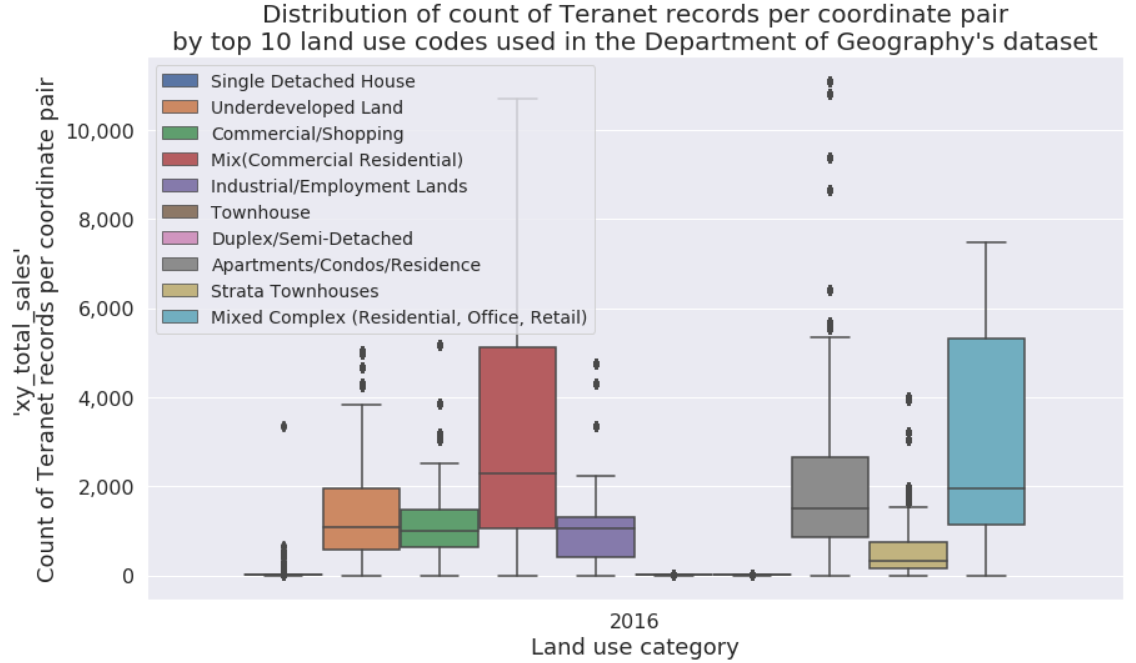
\includegraphics[width=0.98\linewidth,trim=0 0 0 0,clip]{xy_total_sales_dist_by_lu.png}
    \caption{Distributions of total count of Teranet records per coordinate pair by the top 10 land use categories.
    It can be seen that detached houses, duplexes, and townhouses ("collapsed" boxplots) have much lower number of records per coordinate pair.
    It can also be seen that there are some outliers present on the category of detached houses (first boxplot from the left).
    These outliers most likely represent mislabelled records, as it is very unlikely that a detached house can have almost 4'000 sales.}
    \label{fig:xy_total_sales_dist_by_lu}
\end{figure}

The target variable used for the purposes of investigating the possibility of land use classification using the housing market dynamics was constructed by reducing the land use codes found in the Department of Geography's land use dataset.
Department of Geography's land use categories that have the highest counts of Teranet records have been used to reduce all different property types to the three major land use classes.
As many machine learning algorithms are subject to a frequency bias in which they place more emphasis on learning from data observations which occur more frequently, the three classes were selected to have a comparable number of records between themselves to achieve a more balanced dataset.
In addition, chosen groupings combine categories that have a similar distribution of price and count of sales per coordinate pair between land use categories that were grouped together to form a single class.
For example, detached and semi-detached houses and townhouses would have a much smaller frequency of transaction and a higher median price per coordinate pair when compared to condos and strata townhouses.
Figure~\ref{fig:class_2_price_dist} shows an example of such grouping: in class 2, Duplex/Semi-Detached properties are grouped together with Townhouses.

\vspace{5mm}

The three target classes that were introduced are:

\begin{itemize}
    \item Class 0: "condo", including Apartments/Condos/Residence and Strata Townhouses
    \item Class 1: "house", including Single Detached Houses, Duplex/Semi-Detached and Townhouses
    \item Class 2: "other", including Commercial/Shopping, Mix (Commercial Residential), Industrial/Employment Lands, and everything else
\end{itemize}

\begin{figure}[ht]
    \centering
    \begin{subfigure}{\linewidth}
        \centering
        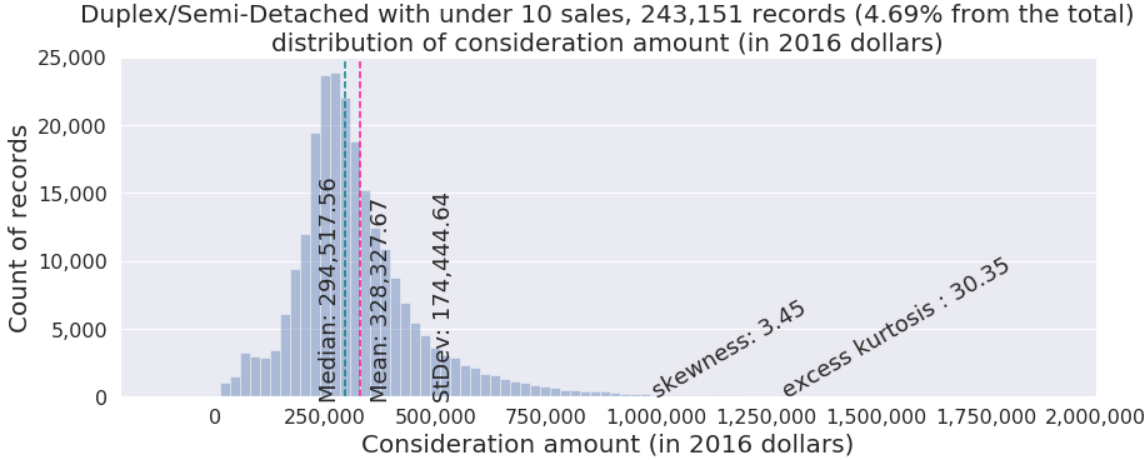
\includegraphics[width=.9\linewidth]{duplex_price_dist.png}
        \label{fig:duplex_price_dist}
        \caption{Duplex/Semi-Detached}
    \end{subfigure}

    \begin{subfigure}{\linewidth}
        \centering
        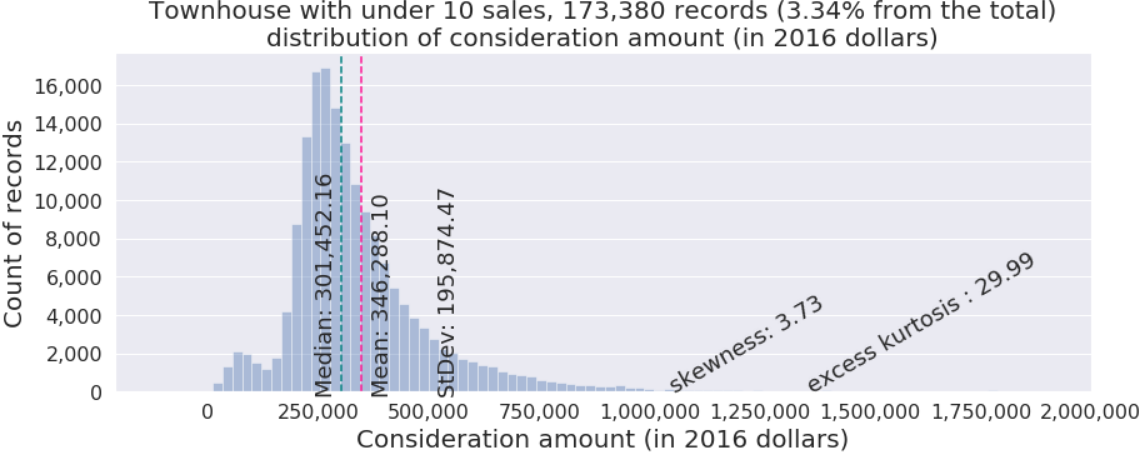
\includegraphics[width=.9\linewidth]{townhouse_price_dist.png}
        \label{fig:townhouse_price_dist}
        \caption{Townhouse}
    \end{subfigure}
    \caption{Distribution of price (in 2016 dollars) for two out of the three property types that are grouped together under Class 2: House.
    Both categories have similar distributions of price and records per coordinate pair between themselves and with the Single Detached Houses, and thus all three categories are grouped together to represent a single class ''house''.}
    \label{fig:class_2_price_dist}
\end{figure}

Classification algorithms, a subcategory of algorithms for supervised learning, predict the discrete unordered categorical class labels of new instances based on past observations.
A trained algorithm is capable of using a set of rules that were learned from past observations to distinguish the new instances between the possible classes.
Once the classes have been determined and assigned, the target variable must be encoded, as it is considered good practice to provide class labels as integer arrays to algorithms to avoid technical glitches and improve computational efficiency.
Class labels are not ordinal and classification estimators in the scikit-learn\cite{scikit-learn} machine learning library in Python treat them as categorical data that does not imply any order.

\section{Missing values} \label{sec:missing_values}

As was mentioned in section~\ref{sec:feature_engineering}, some of the new features engineered from Teranet attributes, such as 'xy\_years\_since\_last\_sale' and 'xy\_years\_to\_next\_sale' contain missing values in each case of the first or the last Teranet record coming from a coordinate pair.
Since classification algorithms cannot handle inputs with missing values, these values were replaced using the following logic:

\begin{itemize}
    \item For all the records with missing 'xy\_years\_since\_last\_sale' (first record from a coordinate pair), values were replaced with the median 'xy\_years\_to\_next\_sale' for this subset (median time interval between all future sales from this Teranet subset).
    \item For all the records with missing 'xy\_years\_to\_next\_sale' (last record from a coordinate pair), values were replaced with the median 'xy\_years\_since\_last\_sale' for this subset (median time interval between all past sales from this Teranet subset).
\end{itemize}

This replacement affects a large number of Teranet records, as there are many coordinate pairs with a low count of records, but this allows the classification algorithm to work on the majority of Teranet data, which improves the generalization of the algorithm and allows classifying land use of most Teranet records.
The features that have missing values also have strong predictive power for land use classes and thus are best kept in the input set with the missing values replaced.
This replacement is done during the fitting of classification algorithm and is not recorded in the final version of Teranet's dataset with new features and keys, were the missing values are left as missing.

\section{Dimensionality reduction} \label{sec:dimensionality_reduction}

Quality of the data plays a critical part in the success of application of a machine learning algorithm, and one of important aspects of data quality is the dimensionality of input space.
The input space may contain features that are either redundant or irrelevant;
highly correlated features also introduce multicollinearity and can make the model unstable, or too sensitive to small changes in the input data.
In machine learning, statistics, and information theory, dimensionality reduction is the process of reducing the number of random variables under consideration;
there is a number of reasons for reducing dimensionality of a dataset:

\begin{enumerate}
    \item reducing the number of features improves computational efficiency and reduces training times
    \item in case of a low signal-to-noise ratio in the dataset, dimensionality reduction can improve the predictive performance of an algorithm\cite{RaschkaMirjalili2017}
    \item simpler models are easier to interpret\cite{James2013}
    \item excessive complexity of the model could cause overfitting\cite{RaschkaMirjalili2017}
    \item the curse of dimensionality\cite{Bellman1954} (in the context of machine learning, the curse of dimensionality describes the phenomena where the feature space becomes too sparse for the size of the training dataset)\cite{RaschkaMirjalili2017}
\end{enumerate}

There is a number of approaches that could be utilized to reduce the dimensionality of the feature space.
There are two main categories of dimensionality reduction techniques:
\begin{itemize}
    \item feature selection, also referred to as Feature Subset Selection, or (FSS), where a subset of the original features is selected
    \item feature extraction, where a new feature subspace is constructed from information derived from the original feature set
\end{itemize}

Feature selection can either be performed manually or by utilizing a feature selection algorithm.
Exhaustive evaluation of all possible feature subsets is computationally unfeasible even for a moderate number of features.
For example, if we are given a feature set with $m = 64$ features and want to reduce it to $n = 11$, an exhaustive evaluation would involve over $10^{12}$ possible feature sets:

\begin{equation}
    _{m}C_n = _{64}C_{11} = \binom{64} {11} = \frac{64!} {11!(64 - 11)!} = 743,595,781,824
\end{equation}

Feature selection algorithms present a practical approach to feature selection at scale;
such algorithms combine a search strategy for proposing new feature subsets with an objective function to evaluate these subsets;
objective function plays the role of a feedback signal used by the search strategy to choose between candidate subset.
Objective functions are divided into three major groups:

\begin{itemize}
    \item filters
    \begin{itemize}
        \item evaluate candidate feature subsets by their information content (e.g., inter/intra class distance, mutual information, etc.)
        \item advantages: have faster execution since there generally is no iterative computation;
        have good generality since they evaluate the intrinsic properties of the data.
        \item disadvantages: tend to select large feature subsets due to monotonic objective functions
    \end{itemize}
    \item wrappers
    \begin{itemize}
        \item use a classifier to evaluate subsets by their predictive accuracy
        \item advantages: have better accuracy since they select subsets based on specific interactions between the classifier and the dataset
        \item disadvantages: slower to execute since a classifier needs to be re-trained multiple times;
        selected feature subset will be specific to the classifier that was used to evaluate the candidate subsets.
    \end{itemize}
    \item embedded methods
    \begin{itemize}
        \item feature selection is performed as a part of model construction process (i.e., LASSO method for constructing a linear model with L1 regularization)\cite{Scikit-learndevelopers2019}
    \end{itemize}
\end{itemize}

A combination of different FSS techniques was applied to reduce the dimensionality of the dataset with Teranet, TTS, and Census variables for classification from 64 to 11 input features.
The first method utilized was SelectFromModel in scikit-learn, a wrapper FSS algorithm that selects an optimal size and composition of a feature subset by fitting the provided classifier to training data and getting the importance weights from the fit model.
SelectFromModel with Random Forest classifier has determined the optimal number of features to be 18;
this number of features was provided to the other FSS algorithms to select the 18 best features from the dataset according to each method.

The second FSS method that was applied to the augmented Teranet dataset comes from the filter family of objective functions: a univariate feature selection algorithm SelectKBest in scikit-learn;
this method selects $k$ highest scoring features based on their scores on the specified univariate statistical test.
Univariate FSS techniques can be useful for better understanding of the data, as they examine each feature individually to determine the strength of its relationship with the target variable.
However, due to this fact, these methods will not necessarily result in improvement in the generalization of a learning algorithm, and thus their results have been used for feature selection in combination with other methods discussed in this section.
The following statistical tests from scikit-learn have been selected for scoring features using SelectKBest FSS algorithm:

\begin{itemize}
    \item Chi-squared stats of non-negative (pre-normalized) features for classification tasks
    \item ANOVA F-value between label/feature for classification tasks
    \item Mutual information for a discrete target
\end{itemize}

The third family of FSS algorithms that were applied were the recursive feature elimination algorithms, wrapper algorithms that evaluate candidate feature subsets and recursively eliminate features until the desired number of dimensions is reached.
RFE class in scikit-learn facilitates feature ranking with recursive feature elimination using the provided external classifier that assigns weights to features.
Another recursive selection method used was the Sequential Backward Selection algorithm implemented as a Python class by Raschka and Mirjalili\cite{RaschkaMirjalili2017}.
Sequential feature selection algorithms are a family of greedy search algorithms that are used to reduce an initial $d$-dimensional feature space to a $k$-dimensional feature subspace where $k<d$.

\begin{figure}[hbt!]
    \centering
    \begin{subfigure}[t]{.45\textwidth}
        \centering
        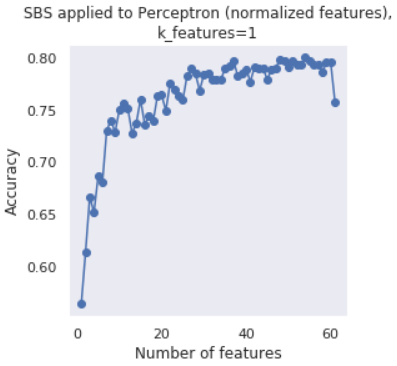
\includegraphics[width=\columnwidth,trim=0 0 0 0,clip]{sbs_perceptron.png}
        \caption{Perceptron}
        \label{fig:sbs_perceptron}
    \end{subfigure}
    ~ %add desired spacing between images, e. g. ~, \quad, \qquad, \hfill etc.
    %(or a blank line to force the subfigure onto a new line)
    \begin{subfigure}[t]{.53\textwidth}
        \centering
        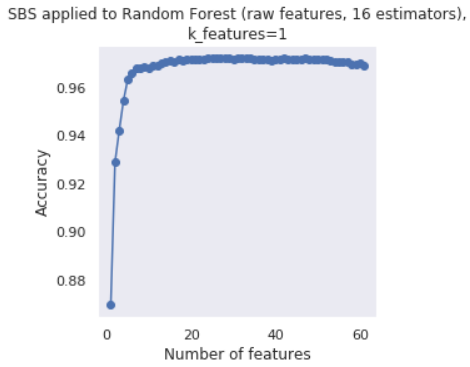
\includegraphics[width=\columnwidth,trim=0 0 0 0,clip]{sbs_forest.png}
        \caption{Random Forest}
        \label{fig:sbs_forest}
    \end{subfigure}
    \caption{Sequential Backward Selection (SBS) is a classic sequential FSS algorithm;
    on each iteration, it eliminates the feature that results in the minimum drop in performance of the provided classifier.
    Figure~\ref{fig:sbs_perceptron} shows SBS run on augmented Teranet dataset with Perceptron and figure~\ref{fig:sbs_forest} shows SBS with Random Forest.
    It can be seen that many features can be eliminated without a significant drop in performance of both classifiers, especially in the case of Random Forest.}
    \label{fig:sbs_teranet}
\end{figure}

Sequential Backward Selection (SBS) is a classic sequential FSS algorithm which aims to reduce the dimensionality of the initial feature subspace with a minimum decay in performance of the classifier;
in some cases of model overfitting, SBS can even improve the predictive power of a classifier.
On each iteration, a feature is removed using the defined criterion function $J$ that we want to minimize;
$J$ can simply be defined as the difference in performance of the classifier before and after a the elimination of a particular feature.
Figure~\ref{fig:sbs_teranet} presents plots produced by running SBS algorithm on augmented Teranet dataset with Perceptron and Random Forest.

As can be seen from the plots produced by SBS, most features in the augmented Teranet dataset can be eliminated without a significant drop in performance of both linear and tree-based models.
As such, final set of features to be used for land use classification was selected by combining the feature subsets selected by each of the FSS methods described above.
Features that have been selected by at least four different methods were selected as the final feature subset that was tested with the classification algorithms and used for final classification of land use;
figure~\ref{fig:top_feats} presents the 11 features that were selected using this logic.

\begin{figure}[hbt!]
    \centering
    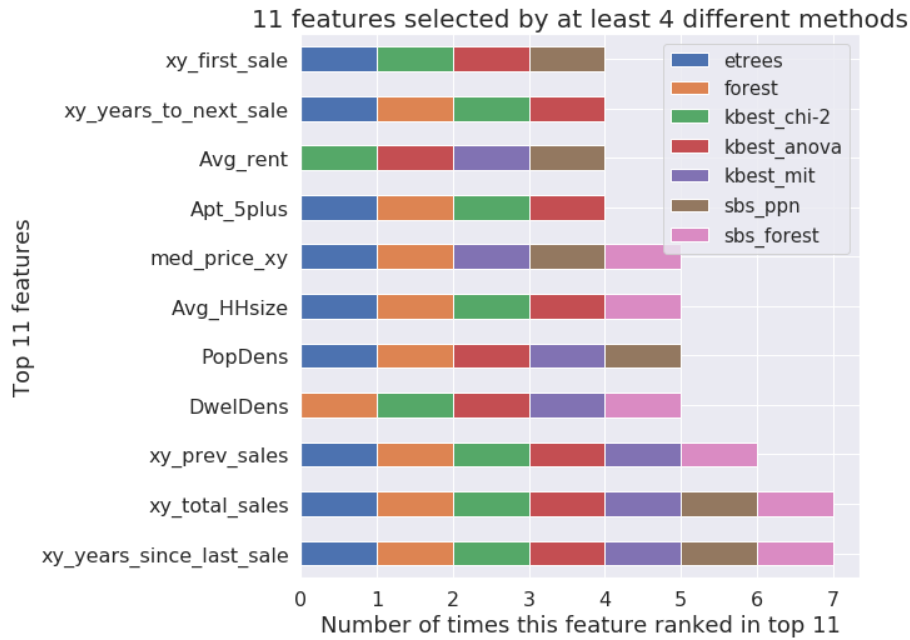
\includegraphics[width=0.7\linewidth,trim=0 0 0 0,clip]{top11f_selection_summary.png}
    \caption{FSS results: 11 features that were selected by at least four different feature selection methods.
    These features were used to select the best-performing model and make the final classification of land use of Teranet records.}
    \label{fig:top_feats}
\end{figure}

From the perspective of embedded feature selection methods, another possible approach to reduce the complexity of a model is to use L1 regularization to penalize large individual weights.
L1 regularization introduces a penalty term to the cost function which is taken as the norm of the weight vector defined as:

\begin{equation} \label{eq:l1_regularization}
    L1:~\norm{\vect{w}}_1 = \sum \limits_{j=1}^m \abs{w_j}
\end{equation}

L1 regularization is similar to L2 regularization, which is defined as:

\begin{equation} \label{eq:l2_regularization}
    L2:~\norm{\vect{w}}_2^2 = \sum \limits_{j=1}^m w_j^2
\end{equation}
where $m$ is the number of features.

However, since in the case of L1 regularization, the sum of squares of weights is replaced with the sum of the absolute values of weights, L1 regularization usually yields sparse feature vectors, since most feature weights will be zero\cite{RaschkaMirjalili2017,Scikit-learndevelopers2019}.
Sparsity of feature vectors can help us get rid of irrelevant features in a high-dimensional dataset;
in this context, L1 regularization can be understood as a technique for feature selection\cite{RaschkaMirjalili2017}.
L1 regularization was attempted with Logistic Regression and Linear Support Vector Classifier models in scikit-learn, but did not result in a significant improvement in model performance.

\section{Tuning model hyperparameters} \label{sec:tuning_hyperparameters}

\textit{To determine whether our machine learning algorithm not only performs well on the training set but also generalizes well to new data, we also want to randomly divide the dataset into a separate training and test set. We use the training set to train and optimize our machine learning model, while we keep the test set until the very end to evaluate the final model. Comparing predictions to true labels in the test set can be understood as the unbiased performance evaluation of our model. In scikit-learn a random split into training and test sets can be quickly computed with the train\_test\_split helper function.}\cite{RaschkaMirjalili2017}

\textit{When evaluating different settings (''hyperparameters'') for estimators, such as the C setting that must be manually set for an SVM, there is still a risk of overfitting on the test set because the parameters can be tweaked until the estimator performs optimally. This way, knowledge about the test set can “leak” into the model and evaluation metrics no longer report on generalization performance. To solve this problem, yet another part of the dataset can be held out as a so-called ''validation set'': training proceeds on the training set, after which evaluation is done on the validation set, and when the experiment seems to be successful, final evaluation can be done on the test set.}\cite{Scikit-learndevelopers2019a}

\textit{However, by partitioning the available data into three sets, we drastically reduce the number of samples which can be used for learning the model, and the results can depend on a particular random choice for the pair of (train, validation) sets.  A solution to this problem is a procedure called cross-validation (CV for short). A test set should still be held out for final evaluation, but the validation set is no longer needed when doing CV. In the basic approach, called k-fold CV, the training set is split into k smaller sets (other approaches are described below, but generally follow the same principles). The following procedure is followed for each of the k “folds”:  A model is trained using  of the folds as training data; the resulting model is validated on the remaining part of the data (i.e., it is used as a test set to compute a performance measure such as accuracy). The performance measure reported by k-fold cross-validation is then the average of the values computed in the loop. This approach can be computationally expensive, but does not waste too much data (as is the case when fixing an arbitrary validation set), which is a major advantage in problems such as inverse inference where the number of samples is very small.}\cite{Scikit-learndevelopers2019a}

Figure~\ref{fig:cross_validation_workflow} presents a typical cross-validation workflow to evaluate model performance as summarized in scikit-learn documentation\cite{Scikit-learndevelopers2019a}.

\begin{figure}[hbt!]
    \centering
    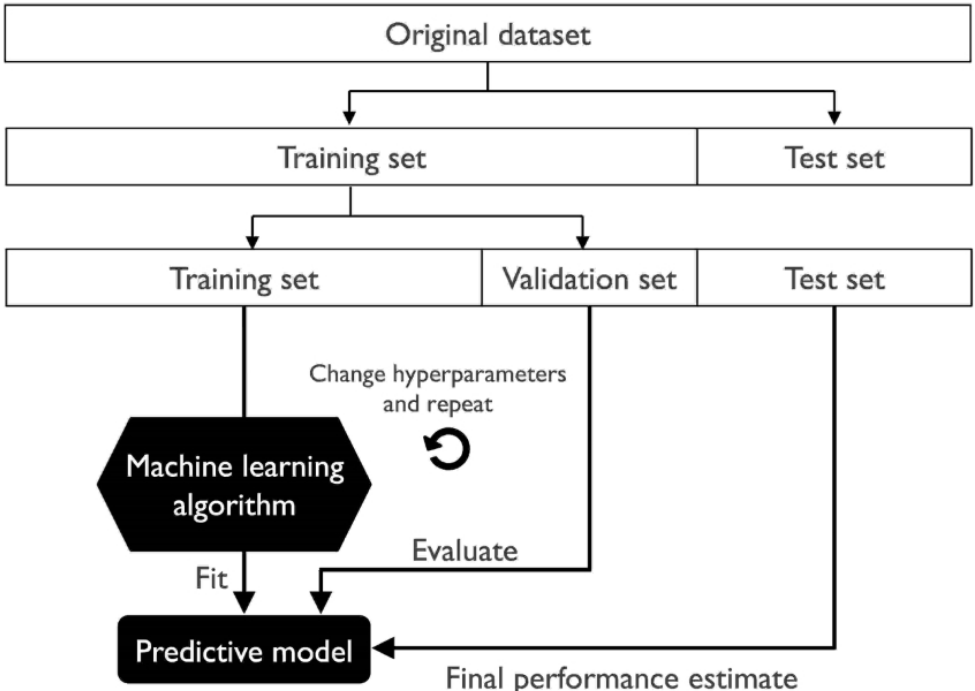
\includegraphics[width=0.7\linewidth,trim=0 0 0 0,clip]{holdout_validation_workflow.png}
    \caption{Holdout cross-validation as summarized by Raschka and Mirjalili\cite{RaschkaMirjalili2017}.}
    \label{fig:holdout_validation_workflow}
\end{figure}

\begin{figure}[hbt!]
    \centering
    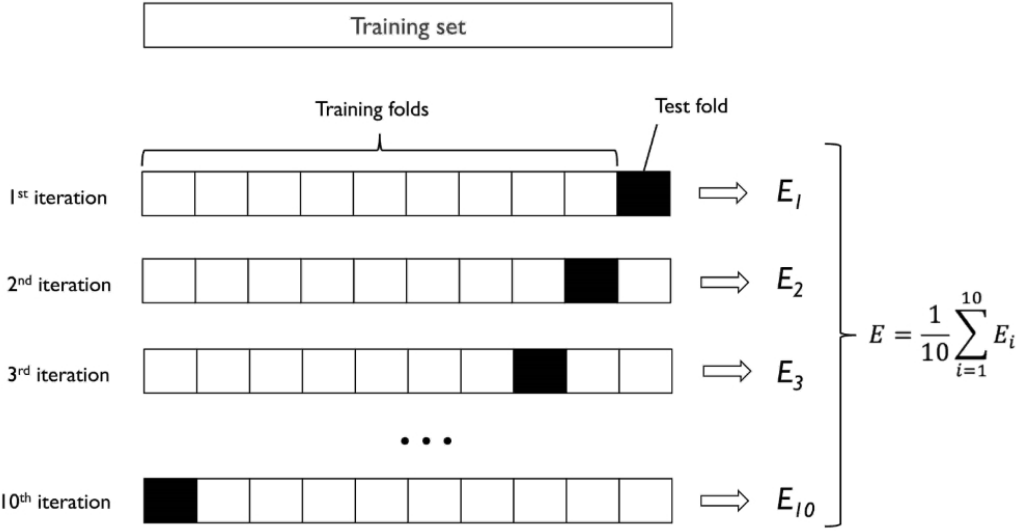
\includegraphics[width=0.8\linewidth,trim=0 0 0 0,clip]{kfold_validation_workflow.png}
    \caption{$K$-fold cross-validation as summarized by Raschka and Mirjalili\cite{RaschkaMirjalili2017}.
    In the case of $K=10$, the training dataset is divided into 10 folds, and during the 10 iterations, nine folds are used for training, and one fold is used as the test set for the model evaluation.
    Estimated performances (for example, classification accuracy or error) for each fold are then used to calculate the estimated average performance E of the model.}
    \label{fig:kfold_validation_workflow}
\end{figure}

\textit{A good standard value for k in k-fold cross-validation is 10, as empirical evidence shows. For instance, experiments by Ron Kohavi on various real-world datasets suggest that 10-fold cross-validation offers the best trade-off between bias and variance (A Study of Cross-Validation and Bootstrap for Accuracy Estimation and Model Selection, Kohavi, Ron, International Joint Conference on Artificial Intelligence (IJCAI), 14 (12): 1137-43, 1995).}\cite{Kohavi1995}

\textit{A slight improvement over the standard k-fold cross-validation approach is stratified k-fold cross-validation, which can yield better bias and variance estimates, especially in cases of unequal class proportions, as has been shown in a study by Ron Kohavi (A Study of Cross-Validation and Bootstrap for Accuracy Estimation and Model Selection, International Joint Conference on Artificial Intelligence (IJCAI), 14 (12): 1137-43, 1995). In stratified cross-validation, the class proportions are preserved in each fold to ensure that each fold is representative of the class proportions in the training dataset}\cite{Kohavi1995}

\textit{For example, each classification algorithm has its inherent biases, and no single classification model enjoys superiority if we don't make any assumptions about the task. In practice, it is therefore essential to compare at least a handful of different algorithms in order to train and select the best performing model. But before we can compare different models, we first have to decide upon a metric to measure performance. One commonly used metric is classification accuracy, which is defined as the proportion of correctly classified instances.}

\textit{After we have selected a model that has been fitted on the training dataset, we can use the test dataset to estimate how well it performs on this unseen data to estimate the generalization error. If we are satisfied with its performance, we can now use this model to predict new, future data. It is important to note that the parameters for the previously mentioned procedures, such as feature scaling and dimensionality reduction, are solely obtained from the training dataset, and the same parameters are later reapplied to transform the test dataset, as well as any new data samples—the performance measured on the test data may be overly optimistic otherwise.}

\textit{randomly partition this dataset into separate test and training datasets is to use the train_test_split function from scikit-learn's model_selection submodule:}

\textit{In this context, stratification means that the train\_test\_split method returns training and test subsets that have the same proportions of class labels as the input dataset.}

\textit{Both the prediction error (ERR) and accuracy (ACC) provide general information about how many samples are misclassified. The error can be understood as the sum of all false predictions divided by the number of total predications, and the accuracy is calculated as the sum of correct predictions divided by the total number of predictions, respectively:}

\begin{equation} \label{eq:prediction_error}
    ERR = \frac{\text{Incorrect classifications}} {\text{Total classifications}}
\end{equation}

The prediction accuracy can then be calculated directly from the error:

\begin{equation} \label{eq:prediction_accuracy}
    ACC = 1 - ERR = \frac{\text{Correct classifications}} {\text{Total classifications}}
\end{equation}

\textit{When dealing with imbalanced data, standard classification metrics do not adequately represent your models performance.}

\section{Feature scaling} \label{sec:feature_scaling}

\textit{Raw data rarely comes in the form and shape that is necessary for the optimal performance of a learning algorithm. Thus, the preprocessing of the data is one of the most crucial steps in any machine learning application. Many machine learning algorithms also require that the selected features are on the same scale for optimal performance, which is often achieved by transforming the features in the range [0, 1] or a standard normal distribution with zero mean and unit variance, as we will see in later chapters.}

\textit{Indeed many estimators are designed with the assumption that each feature takes values close to zero or more importantly that all features vary on comparable scales. In particular, metric-based and gradient-based estimators often assume approximately standardized data (centered features with unit variances). A notable exception are decision tree-based estimators that are robust to arbitrary scaling of the data.}\cite{Scikit-learndevelopers2019b}

\textit{there are two common approaches to bring different features onto the same scale: normalization and standardization.}

\textit{In general, learning algorithms benefit from standardization of the data set. If some outliers are present in the set, robust scalers or transformers are more appropriate.}

\textit{Most often, normalization refers to the rescaling of the features to a range of [0, 1], which is a special case of min-max scaling. To normalize our data, we can simply apply the min-max scaling to each feature column, where the new value x_{norm}^{(i)} of a sample x^{(i)} can be calculated as follows:}

\begin{equation} \label{eq:normalization}
    x_{norm}^{(i)} = \frac{x^{(i)} - x_{min}} {x_{max} - x_{min}}
\end{equation}

Here, $x^{(i)}$ is a particular sample, $x_{\min}$ is the smallest value in a feature column, and  the largest value.

The min-max scaling procedure is implemented in scikit-learn via MinMaxScaler.

\textit{Although normalization via min-max scaling is a commonly used technique that is useful when we need values in a bounded interval, standardization, or mean removal and variance scaling, can be more practical for many machine learning algorithms, especially for optimization algorithms such as gradient descent. The reason is that many linear models, such as the logistic regression and SVM initialize the weights to 0 or small random values close to 0. Using standardization, we center the feature columns at mean 0 with standard deviation 1 so that the feature columns have the same parameters as a standard normal distribution (zero mean and unit variance), which makes it easier to learn the weights. Furthermore, standardization maintains useful information about outliers and makes the algorithm less sensitive to them in contrast to min-max scaling, which scales the data to a limited range of values.}

\textit{standardization, which gives our data the property of a standard normal distribution, which helps gradient descent learning to converge more quickly. Standardization shifts the mean of each feature so that it is centered at zero and each feature has a standard deviation of 1. For instance, to standardize the jth feature, we can simply subtract the sample mean  from every training sample and divide it by its standard deviation :. One of the reasons why standardization helps with gradient descent learning is that the optimizer has to go through fewer steps to find a good or optimal solution (the global cost minimum)}

The procedure for standardization can be expressed by the following equation:

\begin{equation} \label{eq:standardization}
    \vect{x}^{(i)}_{std} = \frac{\vect{x}^{(i)} - \mu_x}{\sigma_x}
\end{equation}

\textit{Here,  is a vector consisting of the jth feature values of all training samples n, and this standardization technique is applied to each feature j in our dataset.}

\textit{we fit the StandardScaler and MinMaxScaler classes only once—on the training data—and use those parameters to transform the test set or any new data point.}

\section{Model selection} \label{sec:model_selection}

\textit{A popular class of procedures for solving classification tasks are based on linear models. What this means is that they aim at dividing the feature space into a collection of regions labelled according to the values the target can take, where the decision boundaries between those regions are linear: they are lines in 2D, planes in 3D and hyperplanes with more features.}

\textit{Trying to understand how the biological brain works, in order to design AI, Warren McCulloch and Walter Pitts published the first concept of a simplified brain cell, the so-called McCulloch-Pitts (MCP) neuron, in 1943 (A Logical Calculus of the Ideas Immanent in Nervous Activity, W. S. McCulloch and W. Pitts, Bulletin of Mathematical Biophysics, 5(4): 115-133, 1943).}

\textit{Only a few years later, Frank Rosenblatt published the first concept of the perceptron learning rule based on the MCP neuron model (The Perceptron: A Perceiving and Recognizing Automaton, F. Rosenblatt, Cornell Aeronautical Laboratory, 1957). With his perceptron rule, Rosenblatt proposed an algorithm that would automatically learn the optimal weight coefficients that are then multiplied with the input features in order to make the decision of whether a neuron fires or not. In the context of supervised learning and classification, such an algorithm could then be used to predict if a sample belongs to one class or the other.}

\textit{The Perceptron is another simple classification algorithm suitable for large scale learning. By default: It does not require a learning rate. It is not regularized (penalized). It updates its model only on mistakes.}

\textit{Logistic regression models the probabilities of an observation belonging to each of the K classes via linear functions, ensuring these probabilities sum up to one and stay in the (0, 1) range. Logistic regression models are typically estimated by maximum likelihood. Although logistic regression is mostly used as an inference tool in tasks where the goal is to understand the role of input variables in explaining the outcome (it produces easily interpretable coefficients, just like linear regression does), it can also prove to be of significant predictive power.}

\textit{Linear Discriminant Analysis (LDA) assumes that the joint densities of all features given target’s classes are multivariate Gaussians with the same covariance for each class. Quadratic Discriminant Analysis (QDA) relaxes the common covariance assumption of LDA through estimating a separate covariance matrix for each class.}

\textit{A Naive Bayes Classifier determines the probability that an example belongs to some class, calculating the probability that an event will occur given that some input event has occurred.}

\textit{let's consider two common ways we'll train a model: tree-based logical rules developed according to some splitting criterion, and parameterized models updated by gradient descent.}

\textit{Machine learning algorithms can be grouped into parametric and nonparametric models. Using parametric models, we estimate parameters from the training dataset to learn a function that can classify new data points without requiring the original training dataset anymore. Typical examples of parametric models are the perceptron, logistic regression, and the linear SVM. In contrast, nonparametric models can't be characterized by a fixed set of parameters, and the number of parameters grows with the training data. KNN belongs to a subcategory of nonparametric models that is described as instance-based learning. Models based on instance-based learning are characterized by memorizing the training dataset, and lazy learning is a special case of instance-based learning that is associated with no (zero) cost during the learning process.}

\textit{Machine learning algorithms can be grouped into parametric and nonparametric models. Using parametric models, we estimate parameters from the training dataset to learn a function that can classify new data points without requiring the original training dataset anymore. Typical examples of parametric models are the perceptron, logistic regression, and the linear SVM. In contrast, nonparametric models can't be characterized by a fixed set of parameters, and the number of parameters grows with the training data. Two examples of non-parametric models that we have seen so far are the decision tree classifier/random forest and the kernel SVM.}

An important point to be summarized from the famous No Free Lunch Theorems (NFL)\cite{Wolpert1996,Wolpert1997} by David H. Wolpert is that no single classifier works best across all possible scenarios, as there is a lack of a priori distinctions between learning algorithms.

\textit{For example, each classification algorithm has its inherent biases, and no single classification model enjoys superiority if we don't make any assumptions about the task. In practice, it is therefore essential to compare at least a handful of different algorithms in order to train and select the best performing model. But before we can compare different models, we first have to decide upon a metric to measure performance. One commonly used metric is classification accuracy, which is defined as the proportion of correctly classified instances.}

\textit{In practice, it is always recommended that you compare the performance of at least a handful of different learning algorithms to select the best model for the particular problem; these may differ in the number of features or samples, the amount of noise in a dataset, and whether the classes are linearly separable or not.}


\textit{Another simple yet more powerful algorithm for linear and binary classification problems: logistic regression. Note that, in spite of its name, logistic regression is a model for classification, not regression.}

\texiit{Logistic regression is a classification model that is very easy to implement but performs very well on linearly separable classes. It is one of the most widely used algorithms for classification in industry. Similar to the perceptron and Adaline, the logistic regression model in this chapter is also a linear model for binary classification that can be extended to multiclass classification, for example, via the OvR technique.}

\textit{Decision trees can build complex decision boundaries by dividing the feature space into rectangles. Decision tree classifiers are attractive models if we care about interpretability. As the name decision tree suggests, we can think of this model as breaking down our data by making a decision based on asking a series of questions. Based on the features in our training set, the decision tree model learns a series of questions to infer the class labels of the samples. Using the decision algorithm, we start at the tree root and split the data on the feature that results in the largest Information Gain (IG). In an iterative process, we can then repeat this splitting procedure at each child node until the leaves are pure. This means that the samples at each node all belong to the same class. In practice, this can result in a very deep tree with many nodes, which can easily lead to overfitting. Thus, we typically want to prune the tree by setting a limit for the maximal depth of the tree. As we can see, the information gain is simply the difference between the impurity of the parent node and the sum of the child node impurities — the lower the impurity of the child nodes, the larger the information gain. Now, the three impurity measures or splitting criteria that are commonly used in binary decision trees are Gini impurity ($I_G$), entropy ($I_H$), and the classification error ($I_E$).}

\textit{Random forests have gained huge popularity in applications of machine learning during the last decade due to their good classification performance, scalability, and ease of use. Intuitively, a random forest can be considered as an ensemble of decision trees. The idea behind a random forest is to average multiple (deep) decision trees that individually suffer from high variance, to build a more robust model that has a better generalization performance and is less susceptible to overfitting.}

1. Draw a random bootstrap sample of size n (randomly choose n samples from the training set with replacement).

2. Grow a decision tree from the bootstrap sample. At each node:

a. Randomly select d features without replacement.

b. Split the node using the feature that provides the best split according to the objective function, for instance, maximizing the information gain.

3. Repeat the steps 1-2 k times.

4. Aggregate the prediction by each tree to assign the class label by majority vote.

\textit{In most implementations, including the RandomForestClassifier implementation in scikit-learn, the size of the bootstrap sample is chosen to be equal to the number of samples in the original training set, which usually provides a good bias-variance tradeoff. For the number of features d at each split, we want to choose a value that is smaller than the total number of features in the training set. A reasonable default that is used in scikit-learn and other implementations is $d=\sqrt{m}$, where m is the number of features in the training set.}

\textit{Although we are growing a very small random forest from a very small training dataset, we used the n\_jobs parameter for demonstration purposes, which allows us to parallelize the model training using multiple cores of our computer (here two cores).}

\textit{k-nearest neighbor (KNN) classifier is particularly interesting because it is fundamentally different from the learning algorithms that we have discussed so far.  KNN is a typical example of a lazy learner. It is called lazy not because of its apparent simplicity, but because it doesn't learn a discriminative function from the training data, but memorizes the training dataset instead. KNN belongs to a subcategory of nonparametric models that is described as instance-based learning. Models based on instance-based learning are characterized by memorizing the training dataset, and lazy learning is a special case of instance-based learning that is associated with no (zero) cost during the learning process.}

The KNN algorithm itself is fairly straightforward and can be summarized by the following steps:

1. Choose the number of k and a distance metric.

2. Find the k-nearest neighbors of the sample that we want to classify.

3. Assign the class label by majority vote.

\textit{The principle behind nearest neighbor methods is to find a predefined number of training samples closest in distance to the new point, and predict the label from these. The number of samples can be a user-defined constant (k-nearest neighbor learning), or vary based on the local density of points (radius-based neighbor learning). The distance can, in general, be any metric measure: standard Euclidean distance is the most common choice. Neighbors-based methods are known as non-generalizing machine learning methods, since they simply “remember” all of its training data (possibly transformed into a fast indexing structure such as a Ball Tree or KD Tree). Being a non-parametric method, it is often successful in classification situations where the decision boundary is very irregular.}\cite{Scikit-learndevelopers2019c}

\textit{Neighbors-based classification is a type of instance-based learning or non-generalizing learning: it does not attempt to construct a general internal model, but simply stores instances of the training data. Classification is computed from a simple majority vote of the nearest neighbors of each point: a query point is assigned the data class which has the most representatives within the nearest neighbors of the point.}

\section{Chapter summary} \label{sec:ml_workflow_summary}
asd